\documentclass[11pt, english, screen]{report-rd-info}
   % - 12pt:  can be preferable to read the report on small screens, ask your supervisors
   % - screen:  to be removed in order to obtain a classical report
\usepackage[latin1]{inputenc}
   % - latin9, utf8, etc.
\usepackage[T1]{fontenc}

% some definitions for the actual contents
\usepackage{enumerate}
\usepackage{color}
\usepackage{amsmath, amssymb}
\usepackage{algorithm,algpseudocode}
%\usepackage{algorithm}
%\usepackage{algorithmic}

\begin{document}

\title{SCAMPLON: A Peer Sampling Service for WebRTC}
\subtitle{A Model and Short Guide}

\authorA{Julian}{Tanke}
\authorB{}{}
\supervisor{Pascal}{Molli}
\cosupervisor{Brice}{Nedelec}
   % In case, there are more than two supervisors, use the following trick:
   %    \cosupervisor{Jean}{Cadre \& {\normalfont Still} Another}
\coordinator{Jos�}{Martinez}
\institution{LINA}
   % - LINA when you're supervised by members of the research teams GRIM or COD (may be some others);
   % - IRCCyN when youre supervised by members of the research team IVC;
   % - XXX when supervised by another organism
   %   (In that case, you have to provide, in the "logos" directories, the files named: XXX.pdf -- if not XXX.jpeg or XXX.png -- for pdflatex *and* XXX.eps for latex);
   % - otherwise comment it
\theme{\'Equipe GRIM}
   % - optionally provide it when an institution has been declared (GRIM, COD or IVC for the local research teams)
   % - otherwise comment it
%\coinstitution{Centre national de la recherche scientifique}{CNRS}{1.7cm}
   % - if you need to add a partner
   % - the logo must be provided, e.g., CNRS.pdf here
   % - the third parameter allows one to control the width of the logo in order to make
   %   it look of the same size of the one from the university of nantes and possibly the laboratory
\date{November 15, 2014}
   % - do not had un 0 in front of the first to ninth day of a mont!
   % - you can altogether ignore the day.

%-------------------------------------------------------------------------------------------------------------

\begin{abstract}
%\small % Comment it out should the abstract by slightly too long to fit in the page.

WebRTC allows web browsers to directly communicate with no server in between which enables massive, distributed applications for the web that are scalable, responsive and failure resistant.
A general paradigm for information dissemination in large distributed systems is the gossip-based communication.
The core of gossiping protocols is the \emph{peer sampling service} that provide every node with random peers to exchange information with.
Peer sampling services do not necessarily rely on global knowledge, instead there are many algorithms that only need local information to provide uniform random samples - for example SCAMP and CYCLON.
This protocols assume that peers are directly addressable - however this is not possible in WebRTC.
Instead, a handshake must be executed over a well-known signaling service whenever a new connection is established.
As a central service significantly decreases the scalability we propose to carry it over into the distributed system - if this is done a node only needs to access the central service to enter the network.
Nodes that are already member of the system can use other peers to function as their signaling service to establish connections to other nodes within the network - this way the protocol stays scalable.

We evaluate CYCLON and SCAMP in a handshaking environment.
Furthermore, we propose SCAMPLON, a new membership protocol composite of parts of SCAMP and parts of CYCLON.
SCAMPLON provides good properties and is not just applicable for WebRTC and handshaking but can also be used more generally as a generic peer sampling service.


   \subsubsection {KEY WORDS}
   Membership management; peer-to-peer; epidemic/gossiping protocols; Scalability; random graphs

\end{abstract}

%\begin{classification}
%   Bibliographic indexing is required. Use the ACM thesaurus:  See \url{http://www.acm.org/about/class/}. (The following example is based on the 1998 version, where general terms and additional key words are optional.)

%   \category{H.2.8}{Database Applications}{Image databases}
%   \category{H.3.3}{Information Search and Retrieval}{Clustering, Information filtering, Relevance feedback}
%   \category{H.3.7}{Digital Libraries}{User issues}
%   \category{I.5.3}{Clustering}{Algorithms, Similarity measures}
%   \category{I.4.10}{Image Representation}{Statistical, Multidimensional}
%   \terms{Algorithms, Performances, Experiments, Human factors, Verification.}
%   \keywords{Content-based image retrieval system, Classification, Feedback loop, Supervised learning.}
%\end{classification}

\maketitle

%--------------------------------------------------------------------------------

%\begin{acknowledgements}
%   The usual place of acknowledgements, if this pleases you or if the work has been conducted as part of a larger endeavour.
%\end{acknowledgements}

%--------------------------------------------------------------------------------

\newpage

\tableofcontents

%--------------------------------------------------------------------------------

%\chapter*{Preface}
%\addcontentsline{toc}{chapter}{Preface}

%TODO
%--------------------------------------------------------------------------------

\chapter{Introduction}

Many efforts have been devoted to establish a data connection between browsers using the WebRTC API\footnote{http://w3c.github.io/webrtc-pc/}. 
Services like PeerCDN\footnote{https://peercdn.com/}, webtorrent\footnote{https://github.com/feross/webtorrent} or Sharefest\footnote{https://www.sharefest.me/} demonstrate how decentralized services now can be deployed easily in web browsers.
This drastically improves the user experience as they can download torrents as easy as watching a youtube video.
However, current solutions do not provide a scalable broadcast.
This, however, is essential for other applications such as distributed collaborative editors or distributed social networks.
Traditionally, gossip protocols are used to implement broadcast in decentralized infrastructure.
This protocols have been used in a various number of large scale systems serving an array of problem settings including information dissemination \cite{Demers:1987:EAR:41840.41841}, information aggregation \cite{Jelasity:2005:GAL:1082469.1082470} and network management \cite{conf/dsom/VoulgarisS03}.
Peers are highly autonomous and independent, which allows the algorithms to be simple when compared to hierarchical approaches.
This protocols can easily scale to millions of peers which can join and leave without significantly disrupting the service.
The hearth of each gossip protocol is its fundamental distributed abstraction: the peer sampling service\cite{Jelasity:2004:PSS:1045658.1045666}.

\section{Statement of the problem}

This raises the problem of deploying gossip algorithms on WebRTC.
Many gossip protocols build up upon the premise that the peers can interconnect easily with each other and, as such, constantly connect to new sets of peers\cite{Voulgaris05cyclon:inexpensive}\cite{Jelasity:2004:PSS:1045658.1045666}.
Unfortunately, certain efforts must be taken to establish a peer-to-peer connection with WebRTC:
as entities in WebRTC cannot directly address each other due to the network layout of the Internet, a handshake, consisting of an offer by one client and a responding answer by the other, must be performed.
This process must be hoist by a well-known service in between, which we will call the \emph{signaling service}.
Furthermore, the handshake potentially changes the communication complexity as connecting to new peers becomes more expansive and error-prone.

\section{Objectives}

In this report we evaluate the cost of two well-known peer sampling services, CYCLON\cite{Voulgaris05cyclon:inexpensive} and SCAMP\cite{Ganesh:2001:SPL:648089.747488}, in a handshaking infrastructure\footnote{Direct addressing is not possible. Instead, a connection between peers must be established over a signaling service}.
We provide a technique to minimize the number of connections to the well-known signaling service, and, 
additionally, we propose SCAMPLON, a new algorithm that merges the advantages of CYCLON and SCAMP regarding network topology and robustness towards handshaking.

\section{Work achieved}

We show that CYCLON can be easily deployed in a WebRTC environment as it only communicates with other nodes in close proximity reducing the handshaking overhead.
We also show that the lease-mechanism in SCAMP can be significantly disturbed under network failure\footnote{See Figure \ref{fig:f_scamp3}}.
We provide a WebRTC library\footnote{https://github.com/justayak/handshake} that allows nodes inside a WebRTC network to host connections between each other without the need of an external service. This minimizes the number of connections towards the signaling service as it is only needed to introduce a new node to an existing network.
Furthermore, we propose an algorithm that combines the good properties of CYCLON and SCAMP and removes some of their problems.
SCAMP is used to enter and remove nodes from the network, thus providing a good random starting distribution and an adaptive partial view size, but uses CYCLON to balance the graph afterwards to exploit its close-proximity exchanges.

\section{Contribution}

Gossip protocols that are designed for the internet have already been introduced by \cite{Ganesh:2003:PMM:642778.642782} and\cite{Voulgaris03arobust}.
However, this protocols assume that a connection can be established with direct addressing, ignoring the limitations mentioned above.
On the other side there are implementations of peer-to-peer networks on top of WebRTC\footnote{http://peerjs.com/} already available. 
Nonetheless they lack truly massive scalability as they rely on a single centralized signaling service to host and maintain the network.
Our contribution is an algorithm, SCAMPLON, that is truly scalable in a WebRTC environment.
Furthermore, the SCAMPLON-protocol is not limited for use in handshaking environments but can also be easily applied in general gossiping algorithms.

\section{Report organisation}

The remainder of this paper is structured as follows: 
Chapter~\ref{chap:Motiv} explains the technology in more depth and provides an example application. 
Chapter~\ref{chap:StateOfTheArt} studies the gossip protocols CYCLON and SCAMP. 
In Chapter~\ref{chap:Proposals}  we will propose SCAMPLON and describe how it differs from the other two protocols.
Chapter~\ref{chap:Experiments} first evaluates the different behaviors of SCAMP and CYCON with handshaking. We than compare SCAMPLON and CYCLON and show that our algorithm provides better overall properties under normal network conditions.
Finally, the conclusion summarises the work and introduce new research issues that are worth pursuing.

%-------------------------------------------------------------------------------------------------------------
\chapter{Background and Motivation}
\label{chap:Motiv}

\section{WebRTC}

Web Real-Time Communications (WebRTC) is a client-side API to enable Real-Time Communications in web browsers \cite{webrtc}.
It is an implementation of SRTP\footnote{Secure Real-time Transport Protocol} with an SDP\footnote{Sockets Direct Protocol} control mechanism on top that can use STUN, TURN and ICE for NAT traversal.

\textit{These APIs should enable building applications that can be run inside a browser, requiring no extra downloads or plug-ins, that allow communication between parties using audio, video and supplementary real-time communication, without having to use intervening servers (unless needed for firewall traversal, or for providing intermediary services).}

As we are interested in sending arbitrary data between peers we will focus on the DataChannel API.
Unfortunately WebRTC cannot create a connection between peers without a signaling service. 
That means that we need some sort of communication exchange (Handshake) prior to the direct peer-to-peer connection.
Figure~\ref{fig:webrtc} demonstrates how a connection is established in WebRTC:

\begin{enumerate}
    \item{Alice needs to find out her public Internet address and her network setup (Routers, Firewall).
To obtain this information, she queries a well-known STUN-Server.}
    \item{To establish a connection with Bob, she now needs to create an offer and send it to the signaling service.}
    \item{The signaling service selects Bob and forwards Alice's offer to him.}
    \item{We assume, that Bob already knows his network setup (as he called a STUN-Server before).
Bob accepts the request that Alice sends to him and wants to communicate. To do so he must create an answer and send it back to Alice. As Bob does not know how to connect to Alice yet, he sends the answer to the signaling service instead.}
    \item{The signaling service sends the answer back to Alice.}
    \item{Upon receiving Bob's positive answer, Alice sends a description of how the communication will be done and how Bob can send data to her. As she does not know how to directly connect to Bob yet, she sends this information to the signaling service.}
    \item{The signaling service forwards Alice's connection information to Bob.}
    \item{Bob checks if he can communicate in any way that Alice suggested, and, if he can, he describes how to connect directly to him. Again, this message is send to Alice through the signaling service.}
    \item{Alice gets the information from Bob and establishes a link to him. From now on they can communicate directly with each other. }
\end{enumerate}

\begin{figure}
    \centering
    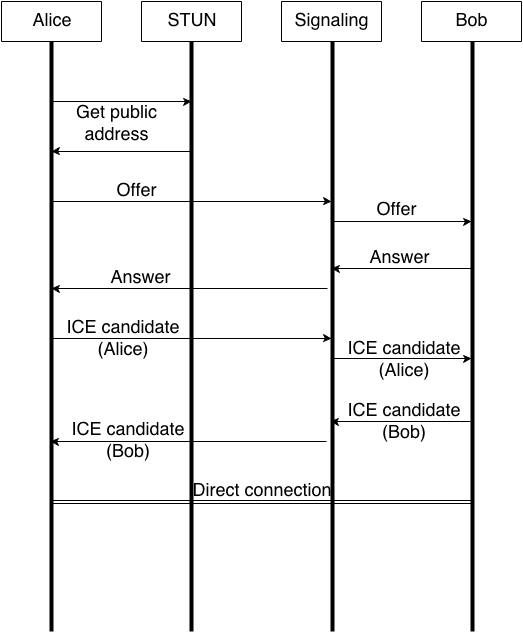
\includegraphics[width=9cm]{Images/WebRTC}
    \caption{Examplary WebRTC connection}
    \label{fig:webrtc}
\end{figure}

\section{Massive Collaborative Editing}

One application for a gossip-based WebRTC network is a massive collaborative editor \cite{nedelec:hal-00921633}\cite{MassCollab} that runs in the web browser.
Unlike current solutions such as Google Docs, Microsoft Word Online or Etherpad we want to support millions of users on one document (e.g. Google Docs only allows 50 users to work on one document).
\cite{MassCollab} describes how parallel editing can scale well with the number of users, implied that some sort of broadcast exists.
However, no assumptions are made about how this broadcast is done.
A centralized service or a fully connected graph do not scale well with the user count.
Instead, using the proposed gossip-based peer-to-peer protocol for WebRTC will make the application more scalable and robust.

%-------------------------------------------------------------------------------------------------------------

% \part{State-of-the-Art} % Comment it out if the state-of-the-art requires several chapters.
                          % Most often, you'll then have a presentation chapter followed by a critical synthesis chapter.
                          % In that case, you must commen tour your work part, hereafter.
% \label{part:StateOfTheArt}

\chapter{State of the Art}
\label{chap:StateOfTheArt}

This chapter introduces fundamental algorithms and concepts. 

\section{Gossip Protocol}

Gossip, also referred to as \emph{epidemic dissemination}, is a  communication protocol initially inspired by observing of how gossips spread in social networks or how diseases spread over a population.
It trades reliability guarantees against scalability properties \cite{Eugster:2003:LPB:945506.945507} and it has been applied to various large scale systems, with the purpose of information dissemination \cite{Demers:1987:EAR:41840.41841}, information aggregation \cite{Jelasity:2005:GAL:1082469.1082470}, network management \cite{conf/dsom/VoulgarisS03} and many more.

The basic idea behind gossip works as follows:
a network is a graph $G=(V,E)$ where $V=\{1,...,n\}$ is a set of $n$ nodes.
Let $E \subset V \times V$ denote neighboring\footnote{In this paper, nodes are considered neighbors if they are directly connected to each other} nodes and let $d_i$ denote the degree of node $i$ in $G$ where 
$d_i$ is constrained by the configuration parameter $c \in \mathbb{Z}_{>0}$ which is called Fanout.
The Fanout defines the number of nodes that are selected when a message is broadcast from a node.
A high value generates a lot of redundant messages while being more fault tolerant and reliable. 
$V$ and $E$ constantly change as nodes leave and join the network and nodes update there neighbors to maintain a uniform distribution.

Assuming a node $i$ wants to broadcast a message $m$ - It sends $m$ to its $d_i$ neighboring nodes. 
A receiving node $j$ evaluates if it already knows $m$ \cite{Koldehofe03buffermanagement} - and if not, it will repeat the previous procedure: broadcast to its $d_j$ neighboring nodes and so forth. 
Usually three types of epidemic dissemination of messages can be distinguished:
\begin{itemize}
    \item \textbf{Push:} When receiving a message, a node sends it to all other nodes in its view.
    \item \textbf{Pull:} A node periodically queries one random other node to check for messages it has not received yet.
    \item \textbf{Push-Pull:} A node sends a message to another random peer and, additionally, queries said peer for data.
\end{itemize}

When $n$ is very large, for a given node $i$ it applies that $d_i << n$.
This is necessary for scalability reasons as, otherwise, the list of neighbors might exhaust a nodes memory and maintaining the list in presence of churn\footnote{Nodes constantly join and leave the network} would be too expansive.
We will call $\mathcal{N}_i \equiv \{j\in V:(i,j)\in E\}$ the \textbf{partial view} of $i$.
The partial view should consist of a random sample of $V$.

\section{Peer Sampling Service}

The peer sampling service \cite{Jelasity:2004:PSS:1045658.1045666}, or, random peer sampling (RPS), is a membership protocol.
The purpose of RPS is to provide each peer with a \emph{uniform sample} of $V$ in a distributed and scalable manner.
It can be used in a variety of gossip-based protocols, for example in topology management \cite{Jelasity:2009:TGF:1570533.1570626}. 
The peer sampling service consists of a simple API:

\begin{itemize}
    \item{\textbf{init:}} Initializes the service on a given node if this has not been done before. This is implementation dependent.
    \item{\textbf{getPeer:}} Returns a peer address if the network contains more than one node. The returned address is a sample drawn from the group. This method can also be used to return multiple random peers, either by providing a paramter $n$ to the function or by simply calling the method multiple times.
\end{itemize}

There are two strategies to maintain partial views in peer sampling services \cite{Leitao_gossip-basedbroadcast} that will play an important role in our evaluation:

\begin{itemize}
    \item{\textbf{Reactive:} The partial view only changes when $V$ changes (Nodes join or leave) and remains stable otherwise.
An example algorithm is SCAMP \cite{Ganesh:2001:SPL:648089.747488}.}
    \item{\textbf{Cyclic:} The partial view is periodically updated every $\bigtriangleup T$ time units and membership information are exchanged with neighbors.
An example algorithm is CYCLON \cite{Voulgaris05cyclon:inexpensive}.}
\end{itemize}

\section{SCAMP}

The probabilistic scalable membership protocol (SCAMP)\cite{Ganesh:2001:SPL:648089.747488} is a reactive peer sampling service.
The size of its local views adapt automatically to a desired value of $(c+1)\log{n}$ where $c$ is a  parameter which specifies the degree of robustness to failure(\cite{Kermarrec:2003:PRD:766617.766623}, \emph{Theorem 1}).
It maintains two separated partial views\cite{Ganesh:2003:PMM:642778.642782}, one for receiving gossip messages (InView $\mathcal{N}^{in}$), one for sending gossip messages (PartialView $\mathcal{N}^{out}$).

If a new node $k$ wants to join the network $G(V,E)$ it needs to have one member $i \in V$ in $\mathcal{N}_k^{out}$ and send a subscription request to $i$.
On receiving a subscription request, $i$ forwards the new peer to all members of its own $\mathcal{N}_i^{out}$, and, additionally, creates $c$ copies of the new subscription and forwards them to randomly chosen nodes in $\mathcal{N}_i^{out}$.
On receiving a forwarded subscription for node $k$, a receiving node $j$ integrates $k$ into its $\mathcal{N}_j^{out}$ with probability $p$ which depends on the size of $\mathcal{N}_j^{out}$ ($p_i=\frac{1}{1+|\mathcal{N}_i^{out}|}$). 
If $j$ does not integrate $k$, it forwards it to another randomly chosen peer from its $\mathcal{N}_j^{out}$.
When a node $i$ decides to keep the subscription of a node $j$, it integrates $j$ into its $\mathcal{N}_i^{out}$ and notifies $j$ to put $i$ into its $InView_j$.
On leaving the network, the leaving node $j$ sends a \emph{replace request} containing a peer from its $\mathcal{N}_j^{out}$ to $|\mathcal{N}_j^{in}|-c$ peers in its $\mathcal{N}_j^{in}$ and a \emph{deleting request} to the remaining ones.
When a node $i$ receives the \emph{replace request} from $j$, it will replace $j$ for the sent peer in its $\mathcal{N}_i^{out}$.

A subscription has a finite lifetime called \emph{lease}\footnote{The lease is implementation dependent: it could be set individually or it could be set globally}.
When expired, the subscribed node will be removed from all PartialViews.
It is a nodes responsibility to resubscribe once its subscription expires.
This mechanic ensures that failed nodes will not remain in the network.
Furthermore, the lease mechanism rebalances the network making it more robust.
Indeed, when a peer joins the system, it only has one node in its partial view, which makes it vulnerable to failures.
However, when peers resubscribe, it adds the link to its inView and therefore, to others partial view.
Hence, even the new peers get subscription requests.

Pseudocode: \cite{Ganesh:2001:SPL:648089.747488}, Section 2.1
\begin{algorithm*}[!htbp]
    \caption{Subscription management in SCAMP}
    \begin{algorithmic}[1]
        \Procedure{OnSubscribe}{$subscriber$}
        \For{each $peer$ in $\mathcal{N}^{out}$}
        \State send \textbf{forwardedSubscription} with $subscriber$ to $peer$
        \EndFor
        \For{each $peer$ in sample($\mathcal{N}^{out}$, $c$)}
        \State send \textbf{forwardedSubscription} with $subscriber$ to $peer$
        \EndFor
        \EndProcedure
    \end{algorithmic}
    \label{alg:scamp1}
\end{algorithm*}

\begin{algorithm*}[!htbp]
    \caption{Handling of a forwarded subscription in SCAMP}
    \begin{algorithmic}[1]
        \Procedure{OnForwardedSubscription}{$subscriber$}
        \State $keep \gets$ randomChoiceBetween0and1()
        \State $keep \gets \lfloor (|\mathcal{N}^{out}| + 1) * keep \rfloor$
        \If{$keep \equiv 0 $ and $subscriber \notin \mathcal{N}^{out}$}
        \State 
        \State // potentially very expensive as the handshake must be traced over
        \State // possibly many hops
        \State $\mathcal{N}^{out} \gets \mathcal{N}^{out} \cup \{subscriber\}$
        \State
        \Else
        \State $peer \gets$ sample($\mathcal{N}^{out}$, $1$)
        \State send \textbf{forwardSubscription} with $subscriber$ to $peer$
        \EndIf
        \EndProcedure
    \end{algorithmic}
    \label{alg:scamp2}
\end{algorithm*}

\subsection{Indirection}

In SCAMP, good scaling behavior is ensured when new nodes select their entry point uniformly random among the existing members\footnote{\cite{Ganesh:2001:SPL:648089.747488}, 3.1}.
However, in reality this is seldom the case. Instead it can be expected that few nodes will be designated entrances into the network.
To ensure a random distribution under this circumstances SCAMP introduces \emph{indirection} where the initial entrance node forwards the subscribers request to a node that is approximately chosen at random among the existing nodes.
This is done by a random walk\footnote{the exact algorithm is out of the scope of this report} of length $\log{n}$ which is the expected diameter of the graph.

% +++++++++++++++++++++++++++++++++++++++++++++++++++++++++++=++++++++++++++
% +++++++++++++++++++++++++++++++++++++++++++++++++++++++++++=++++++++++++++
\section{CYCLON}

CYCLON \cite{Voulgaris05cyclon:inexpensive} is a cyclic peer sampling service.
Each peer maintains a partial view of size $c$ and repeatedly exchanges its view with a neighbor - this operation is called a shuffle.
The protocol works as follows\footnote{Enhanced Shuffling, described in \cite{Voulgaris05cyclon:inexpensive}}:

Every $\bigtriangleup T$ time unit a node $i$ executes the shuffle function:

\begin{enumerate}
    \item{Increase by one the age of all neighbors.}
    \item{Select neigbor $j$ with the highest age among all neighbors, and $l-1$\footnote{$1 \le l \le c$}} other random neighbors.
    \item{Replace $j$'s entry with a new enty of age 0 and with $i$'s address.}
    \item{Send the updated subset to peer $j$}
    \item{Receive from $j$ a subset of no more than $t$ of its own entries.}
    \item{Discard entries pointing at $j$ and entries already contained in $i$'s partial view.}
    \item{Update $i$'s partial view to include all remaining entries, by firstly using empty slots (if any), and secondly replacing entries among the ones sent to $j$}
\end{enumerate}

On receiving the shuffle request from $i$ at $j$, $j$ sends back a random subset of $l$ of its neighbors and updates its own partial view with the sent data but it does not increase the age of the items in the partial view.
When a node $i$ does not get a response from a node $j$ after it sent a shuffle request it will discard node $j$ from its partial view as it seems to be failed. 
Because of this, failed nodes will be removed from the network in bounded time.
As in SCAMP, if a node wants to join the network, it needs to know another node that is already part of it.

\begin{algorithm*}[!htbp]
    \caption{Active thread in CYCLON}
    \begin{algorithmic}[1]
        \While{termination condition not reached}
        \State wait $\bigtriangleup T$
        \State $partialView \gets$ increaseAge($partialView$)
        \State $peer \gets$ max(orderByAge($partialView$))
        \State $rand \gets $ sample($partialView \backslash \{peer\}$ , $l-1$) $\cup \{$[addr:$ownAddress$, age:$0$]$\}$
        \State send $rand$ to $peer$
        \State $otherRand \gets $ receive from $peer$
        \State $otherRand \gets otherRand \backslash \{partialView \cup \{[addr:ownAddress, age:*]\}\}$
        \State $partialView \gets partialView \backslash rand$
        \State
        \State // this part is very expensive with handshake
        \State $partialView \gets partialView \cup otherRand$
        \State
        \While{$|partialView| < c$}
        \State // shift removes the first element of an list
        \State $partialView \gets shift(orderByAge(rand))$
        \EndWhile
        \EndWhile
    \end{algorithmic}
    \label{alg:cyclon1}
\end{algorithm*}

\begin{algorithm*}[!htbp]
    \caption{Passive thread in CYCLON}
    \begin{algorithmic}[1]
        \Procedure{OnExchange}{$peer$, $otherRand$}
        \State $rand \gets$ sample($partialView$, $l$)
        \State send $rand$ to $peer$
        \State $otherRand \gets otherRand \backslash partialView$
        \State $partialView \gets partialView \backslash rand$
        \State
        \State // this part is very expensive with handshake
        \State $partialView \gets partialView \cup otherRand$
        \State
        \While{$|partialView| < c$}
        \State // shift removes the first element of an list
        \State $partialView \gets shift(orderByAge(rand))$
        \EndWhile
        \EndProcedure
    \end{algorithmic}
    \label{alg:cyclon2}
\end{algorithm*}


% +++++++++++++++++++++++++++++++++++++++++++++++++++++++++++=++++++++++++++
% +++++++++++++++++++++++++++++++++++++++++++++++++++++++++++=++++++++++++++




% +++++++++++++++++++++++++++++++++++++++++++++++++++++++++++=++++++++++++++
% +++++++++++++++++++++++++++++++++++++++++++++++++++++++++++=++++++++++++++

\section{Synthesis}

The main goal for using gossip based algorithms with WebRTC is to allow the Network to scale to vast sizes.
To fulfill this properties the protocol needs to relay (mostly) on local information and make use of a partial view that adapts automatically to the full network size to guaranty efficient information dissemination.
Additionally, as the system needs to employ handshaking due to WebRTC, the protocol must reduce the number of messages needed to establish a connection between two nodes.
This is important as each additional node in between reduces the probability of successfully establish a connection.
This restriction implies that nodes for exchanging information should be chosen from the temporary close neighborhood.
Table~\ref{tab:Comparison} shows that the two introduced algorithms each provide one feature while lacking the other.

\hfill \break
\begin{tabular}{l | c r }
 properties & SCAMP & CYCLON \\
  \hline
  adaptive size & \textcolor{green}{Yes} & \textcolor{red}{No} \\
  close proximity to neighbors & \textcolor{red}{No} & \textcolor{green}{Yes} \\
  divergence speed & slow & fast \\
  \label{tab:Comparison}
\end{tabular}
\hfill \break

Furthermore, we want the algorithm to diverge all its partial view sizes to the optimal value as fast as possible. 
Here, CYCLON is clearly better as its $\bigtriangleup T$ can be much smaller than the lease time in SCAMP allows.

\section{Conclusion}

All mentioned algorithms have certain problems and limitations when handshaking is added.
In CYCLON the value of $\bigtriangleup T$ must be higher than the time the peers need to connect.
This could be implemented by setting $CONNECTION-TIMEOUT < \bigtriangleup T$.
This will increase the time a news will take to be fully disseminated into the network by constant time.
We show that, other than that, the protocol remains relatively stable and performs reliable as the added overhead is only constant.

SCAMP, on the other hand, must employ more complex engineering as its connecting contract is much more complicated.
The added complexity for SCAMP is not constant but rather depending on the network size.
This results in SCAMP being more fragile which is even increased by its lease-mechanism which can be shown in our experiments (\ref{fig:f_scamp1}).


% +++++++++++++++++++++++++++++++++++++++++++++++++++++++++++=++++++++++++++
% +++++++++++++++++++++++++++++++++++++++++++++++++++++++++++=++++++++++++++


%--------------------------------------------------------------------------------

% \part{Proposals} % Commet it out if this has been done for the state-of-the-art
% \label{part:Proposals}

\chapter{Proposals}
\label{chap:Proposals}

Our research question states: \emph{What is the cheapest handshake gossip algorithm?}
We consider an algorithm to be cheaper than another, if, on average, it employs less handshakes and as few open connections as possible.
This also counts the number of peers in an \emph{intermediate handshake}.
We consider a handshake to be \emph{intermediate} if a peer $i$ cannot directly hoist a connection between two nodes $a$ and $b$ but instead needs to apply $m, m < 0$ intermediate nodes to establish a connection.
This is necessary due to the requirement to reduce the connections to a centralized signaling server as much as possible and, instead, use the decentralized peer-to-peer network to carry out the signaling service, as soon as a node is member of the system.
Additionally, we want our partial view to stay adaptive towards the network size.

\section{Combining SCAMP and CYCLON: SCAMPLON}

We propose to combine SCAMP and CYCLON into one protocol to exploit both its advantages and to remove both its issues.
SCAMP will be used to introduce new peers into the network and to remove them if they wish to leave.
Instead of SCAMP`s lease mechanism CYCLON`s shuffle protocol will take over and balance out the partial views.
To allow this, the aging process from CYCLON is applied.
As the protocol cannot rely on constant values for $c$ and $l$ from CYCLON anymore those need to be calculated on the fly: $l = \left \lceil{\frac{|partialView|}{2}}\right \rceil$,
SCAMP guarantees that $|partialView| \geq 1$.
The partial view size $c$ might change whenever a shuffle is performed as the algorithm will adapt its size towards the neighbor it exchanges data with.
It is defined by the size of the partial view subtracted by the size of the subset sent to the partner peer plus the size of the subset received from the partner peer. 
In the long run, this will result in all peers having similar sized partial views. 

Suppose that node $a$ wants to exchange its partial view with node $b$ and that the graph is created with the previously described SCAMP algorithm. 
The resulting partial view at $a$ must be of size $c_a = |partialView_a| - l_a + l_b$ while the partial view of $b$ must be of size $c_b = |partialView_b| - l_b + l_a$ after the shuffling process.
Nodes with an even initial partial view size will have $\left \lceil{\frac{|a|+|b|}{2}}\right \rceil$ peers in the resulting view while nodes with an odd sized initial partial view will have a new view with length $\left \lfloor{\frac{|a|+|b|}{2}}\right \rfloor$.

A remarkable difference regarding CYCLON is that it is explicitly allowed to have the same node multiple time in ones partial view. 
On the other hand, it must be ensured that, after each shuffle, the partial view has exactly the size as described above.
This is important to keep the number of arcs in the graph constant to the value created by SCAMP. 

\begin{enumerate}
    \item Increase by one the age of all neighbors.
    \item{Select neighbor $b$ with the highest age among all neighbors, and $l_a-1$ other random neighbors.}
    \item{Replace $b$'s entry with a new enty of age 0 and with $a$'s address.}
    \item{Send the updated subset to peer $b$}
    \item{Receive from $b$ a subset of $l_b$ random peers from its partial view.}
    \item{Exchange entries pointing at $b$ with nodes that were previously send to $b$ (ordered by age). If not enough nodes are available to exchange all arcs pointing to $a$ create new entires that point to $b$. It is essential that the size of this set does not change.}
    \item Remove $b$ and the $l_a-1$ sent peers from $a$`s partial view. 
    \item{Join together the remaining partial view and add the updated received list sent from $b$. If the partial view was odd at the beginning it must be of size $\left \lceil{\frac{|a|+|b|}{2}}\right \rceil$ now, otherwise $\left \lfloor{\frac{|a|+|b|}{2}}\right \rfloor$.}
\end{enumerate}

The basic algorithm to connect a node to the network is described in the previous chapter about SCAMP in Algorithm \ref{alg:scamp1} and Algorithm \ref{alg:scamp2}.
The algorithms for shuffling are described in Algorithm \ref{alg:scamplon1} and Algorithm \ref{alg:scamplon2}.

%--------------------------------------------------------------------------------
\section{Connectivity}

As the protocol is based on CYCLON it also inherits CYCLONS connectivity properties\footnote{\cite{Voulgaris05cyclon:inexpensive}, 3.1.} that states that, given a fail-free environment, the connectivity of the network is guaranteed.
That means that no node becomes disconnected as a result of a shuffling operation.
We show that even with the variable partial view size the graph stays connected when subject to an shuffle:

\begin{figure} [H]
    \centering
    \includegraphics[width=8cm]{Images/graphs/ex1}
    \caption{Shuffle from $a$ to $b$. The left graph represents before and the right graph represents after the shuffle. The link is inverted and $b$ transfers some of its peers to $a$.}
    \label{fig:ex1}
\end{figure}

When two nodes shuffle, the connecting arc is inverted. 
Additionally, the bigger\footnote{the node with more elements in its partial view} peer will transfer some of its node to the smaller one to seek for an size equilibrium. 

When two subsets $A$ and $B$ are connected by at least one link, the link will be passed around inside the subsets keeping the subsets connected or will simply invert when the linked nodes shuffle thous keeping the graph connected.

We can also show that the property of holding multiple links to the same peer, as described in figure \ref{fig:ex2}, will not affect the overall network in the long run.

\begin{figure} [H]
    \centering
    \includegraphics[width=8cm]{Images/graphs/ex2}
    \caption{Shuffle from $a$ to $b$. The left graph represents before and the right graph represents after the shuffle. The link is inverted and $b$ and $a$ exchanged random peers.
    $a$ must keep alive all the links, even though they point to the same node.}
    \label{fig:ex2}
\end{figure}

The graph stays connected as no link is destroyed. 
The double connection will be resolved eventually as $c$`s entries in $a$`s partial view age over time which will result in $a$ exchanging partial views with $c$. As $c$ cannot hold links to itself, $a$ will be supplied by a fresh set of peers different from $c$.

When two nodes reference each other we call this a loop (A loop is described in figure \ref{fig:ex3}).
We must show that they will ultimately be resolved as they yield undesirable properties regarding the clustering coefficient which badly impacts the resilience of the graph towards network failure. 

Fortunately, loops can be broken both from within the loop as well as from outside.
In the internal break, one of the loop peers $p_{loop}$ has other non-looping members in its partial view. 
In deterministic (~ $\log{n}$ shuffles) time, this non-looping node will be selected for shuffling.
This potentially removes some or all looping arcs from $p_{loop}$.
Alternatively, the outside link can be passed inside the loop and potentially replace the pointers that create the loop.

\begin{figure} [H]
    \centering
    \includegraphics[width=8cm]{Images/graphs/ex3}
    \caption{Shuffle from $a$ to $b$. An external node breaks the loop.}
    \label{fig:ex3}
\end{figure}

When at least one member of the loop is inside a partial view from another peer inside the graph, the loop can be broken from outside, as described in figure \ref{fig:ex3}.
The external link potentially replaces one looping link thus either reducing or removing the loop. 

\section{Handshaking}

As we want to use SCAMPLON in a WebRTC environment we must evaluate its behavior when applied to handshaking.
As our tests show, SCAMP`s lease mechanism breaks when handshaking is involved and a perfect network cannot be guaranteed.
On the other hand, CYCLON just adds a constant overhead on top of its complexity but otherwise stays resistant towards network failure letting it perform similar to its non-handshaking implementation.
When facing a potentially erroneous network it is advised to use a $c$ value $c>0$ for the introduction part of SCAMPLON to ensure that the number of arcs is around $(c+1) n\log{n}$.
After the hurdle of introduction is solved, handshaking will play only a minor role as the CYCLON`ic part of the protocol will take over which is more adapted towards handshaking because it only makes use of neighbors in close proximity.

\begin{algorithm*}[!htbp]
    \caption{Active thread in SCAMPLON}
    \begin{algorithmic}[1]
        \While{Termination condition not reached}
        \State wait $\bigtriangleup T$
        \State $l \gets \max \{\left \lceil{\frac{|partialView|}{2}}\right \rceil, 1\}$
        \State $p \gets $ the peer of this node
        \State $partialView \gets$ increaseAge($partialView$)
        \State $q \gets$ max(orderByAge($partialView$))
        \State $sample \gets$ sample($partialView\backslash\{q\}$,$l-1$) $\cup \{$node: $p$, age:$0\}$
        \State send $sample$ to $q$
        \State $sample` \gets $ receive from $q$
        %\If{$s$ is even}
        %\State $s`` \gets \left \lceil{\frac{s+s`}{2}}\right \rceil$
        %\Else
        %\State $s`` \gets \left \lfloor{\frac{s+s`}{2}}\right \rfloor$
        %\EndIf 
        \State $partialView \gets partialView \backslash sample$
        \If {$p \in sample`$}
        \State $sent \gets sample \backslash \{\{$node: $p $ age:$*\}, \{$node: $q$, age: $*\} \}$
        \State $sizeBefore \gets |sample`|$
        \State $sample` \gets sample`\backslash \{$node: $p $ age:$* \}$ // remove all possible links to our node
        \State $removeCount \gets sizeBefore - |sample`|$
        \For {$i \rightarrow removeCount$}
        \If {$|sent| > 0$}
        \State $sample` \gets sample` \cup $ pop(orderByAge($sent$)) // fill up with the youngest items
        \Else
        \State $sample` \gets sample` \cup \{ $node:$q $ age: $0\}$ // create new links to the oldest node
        \EndIf
        \EndFor
        \EndIf
        \State $partialView \gets partialView \cup sample`$
        \EndWhile
    \end{algorithmic}
    \label{alg:scamplon1}
\end{algorithm*}

\begin{algorithm*}[!htbp]
    \caption{Passive thread in SCAMPLON}
    \begin{algorithmic}[1]
        \Procedure{OnExchange}{$p$, $q$, $sample`$} // $p$ = local peer, $q$ = sending peer, $sample`$ = sample of $q$`s partial view
        \State $l \gets \max \{\left \lceil{\frac{|partialView|}{2}}\right \rceil, 1\}$
        \State $sample \gets$ sample($partialView$, $l$)
        \State send $sample$ to $peer$
        \State $partialView \gets partialView \backslash sample$
        \If {$p \in sample`$}
        \State $sent \gets sample \backslash \{\{$node: $p $ age:$*\}, \{$node: $q$, age: $*\} \}$
        \State $sizeBefore \gets |sample`|$
        \State $sample` \gets sample`\backslash \{$node: $p $ age:$* \}$ // remove all possible links to our node
        \State $removeCount \gets sizeBefore - |sample`|$
        \For {$i \rightarrow removeCount$}
        \If {$|sent| > 0$}
        \State $sample` \gets sample` \cup $ pop(orderByAge($sent$)) // fill up with the youngest items
        \Else
        \State $sample` \gets sample` \cup \{ $node:$q $ age: $0\}$ // create new links to the other node
        \EndIf
        \EndFor
        \EndIf
        \State $partialView \gets partialView \cup sample`$
        \EndProcedure
    \end{algorithmic}
    \label{alg:scamplon2}
\end{algorithm*}


%--------------------------------------------------------------------------------

%\part{Experiments and Results} % in case of several chapters, then name the chapters differently
%\label{part:Experiments}

\chapter{Experiments and Results}
\label{chap:Experiments}

All simulations were conducted using PeerSim Simulator\footnote{http://peersim.sourceforge.net/}. 
Existing implementations of CYCLON and SCAMP could be used and adapted for handshaking-based simulation.

The first part of the experiment revolves around handshaking with CYCLON and SCAMP while the second part of the  experiments compares the new algorithm SCAMPLON with CYCLON.

We define a \emph{cycle} to be the time period during which all nodes executed one gossiping function, which are defined more precisely in Algorithm \ref{alg:scamp1}, \ref{alg:scamp2}, \ref{alg:cyclon1}, \ref{alg:cyclon2}, \ref{alg:scamplon1} and \ref{alg:scamplon2}.
From this follows that it takes two cycles in CYCLON to complete a shuffle - the first cycle handles the shuffle initialization (\ref{alg:cyclon1}), the second cycle handles the shuffle response (\ref{alg:cyclon2}).
SCAMP on the other hand needs a minimum of three cycles to complete a subscription: the first cycle handles indirection, the second one the subscription (\ref{alg:scamp1}) and the last one handles the multiple forwarded subscriptions (\ref{alg:scamp2}).
However, SCAMP`s subscription can easily consume more than three cycles as both recursive functions, indirection as well as forward, greatly depend on the network size and thus may include more hops and, as such, more cycles.

Peers communicate between each other with messages.
We also test the behavior of the algorithms against a specific failing quota of these messages meaning that a certain percentage of them will not reach their target peer.
With this experiments we hope to get some insight into the failure resistance of the different protocols.

\section{Handshaking}

In this section we will compare SCAMP and CYCLON with their handshaking counterparts.
We want to evaluate how handshaking influences the algorithms properties.
Furthermore, we want to find out what error rates can be tolerated by the handshaking implementations.
The experiments with CYCLON are done with $c = 20$ and $l = 8$ while the experiments with SCAMP are done with $c=2$.
All simulations where run with $1000$ nodes.
The network is initialized as a line, that means: $n_0$ is connected to $n_1$ is connected to $n_2$ and so on.

\subsection{Convergence}

We want to evaluate how fast SCAMP and CYCLON converge to their ideal properties, given that both algorithms are initialized in non-optimal ways.

We use two metrics to determine if a network is converged or not: the \emph{clustering coefficient} and the \emph{average path length}.
In the following we describe the experiments in more detail:

\subsubsection{Clustering Coefficient}

% OBJECTIVE
The \emph{clustering coefficient} is a measure for a graphs tendency to contain cliques as well as for its transitivity.
We calculate the average clustering coefficient by summing together all local clustering coefficients which then gets divided by the number of nodes $n$. 

$\bar{C} = \frac{1}{n}\sum\limits_{i=1}^{n} C_i$

% DESCRIPTION

The local clustering coefficient $C_i$ defines how close a node and its immediate neighbors are to be a clique.

In general, it is not desired for a peer-to-peer network to have a high average clustering coefficient as it weakens the connectivity of the cluster to the rest of the graph which increases the chance of partitioning.
Another disadvantage of a highly clustered network is that information dissemination will be more redundant.

% RESULT

Figure \ref{fig:cluster_cyclon3} shows the average clustering coefficient with CYCLON, run over $2500$ cycles. The x-axis shows the average cluster coefficient while the y-axis shows the number of cycles.
Both implementations, with and without handshaking, behave very similar when no network errors occur.
It should be noted that the handshaking algorithm converges towards a slightly higher limit than the non-handshaking version.
When network errors are introduced, the handshaking variant degrades faster than the non-handshaking version.


\begin{figure}[H]
    \centering
    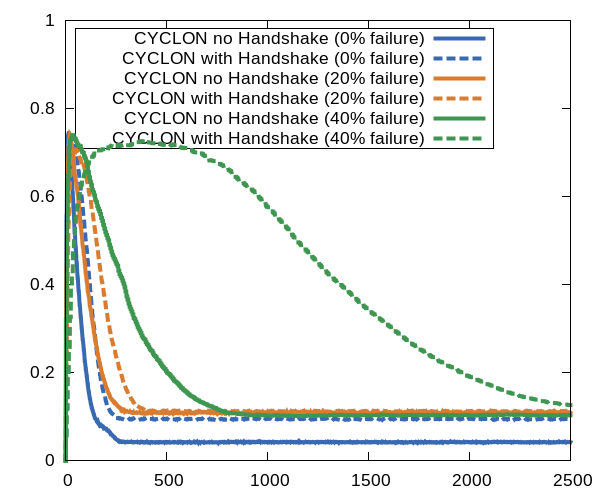
\includegraphics[width=9cm]{Images/statistics/cyclon_1000_c20/all}
    \caption{average clustering of the CYCLON protocol.
    The x-axis denotes the number of cycles while the y-axis denotes the cluster coefficient.}
    \label{fig:cluster_cyclon3}
\end{figure}

Figure \ref{fig:cluster_scamp3} show the average clustering coefficient with SCAMP, run over $100000$ cycles (note that the x-axis is scaled by $(* 100)$).
The first thing to note is that SCAMP needs notably more cycles to converge than CYCLON.
While CYCLON converges after roughly 200 cycles, SCAMP fully converges only after around 20000 cycles.

\begin{figure}[H]
    \centering
    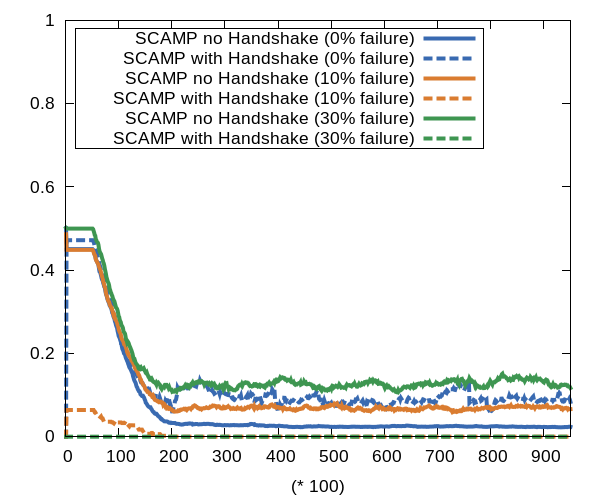
\includegraphics[width=9cm]{Images/statistics/scamp_1000_c2/cluster/all}
    \caption{average clustering of the SCAMP protocol. The x-axis denotes the number of cycles while the y-axis denotes the cluster coefficient.}
    \label{fig:cluster_scamp3}
\end{figure}

SCAMP relies on its lease mechanism to rebalance the graph where a node has a certain lifespan and, after the lifespan is over, it gets removed from other peers view, removes itself from the network and reintroduces itself through a node in its partial view.

SCAMP with handshaking converges slightly slower and to a higher value than the non-handshaking version when all messages are delivered.
However, when errors are introduced, the handshaking version yields lower values than its non-handshaking version.
When the error rate is set to 30\% SCAMP`s handshaking version does not deliver any useful values anymore.

% REASON

There are several explanations for the results: as handshaking needs more hops, heck has more sources of error, it is expected that those versions perform worse than the non-handshaking protocols meaning that they take longer to converge to optimal properties and that their optimal properties are not as good as those generated with non-handshaking protocols.
CYCLON`s results perfectly follow these expectations even when network failure is present.
It can be stated that handshaking CYCLON behaves robust and very similar to its non-handshaking counterpart.
Furthermore, it converges to its ideal state relatively fast as few cycles are needed to fill up a peers partial view.
When the partial views are filled up CYCLON can be considered random thus providing properties of random graphs. 
SCAMP`s non-handshaking version provides good results even when network errors are present.
Furthermore, it converges to a smaller average clustering coefficient than CYCLON, which is preferred.
This can be explained by the smaller number of peers in its partial views: as there are fewer interconnections there are also fewer redundant connections thus there are less cliques.
In contrast, SCAMP converges very slowly (after around 20000 cycles) when compared to CYCLON as its lifespan must be selected carefully to avoid large chunks of the network to leave in parallel. 
In the simulation we obtained this behavior by assigning random values over a range that is bigger than the number of peers.
Handshaking with SCAMP, on the other hand, does not does not adapt to message loss.
Even with low failure rates the graph quickly degrades until it is not connected anymore.
Another observation is that the handshaking SCAMP becomes unreliable when network errors are introduced.
The reason for this is that, with every lease and join on average more arcs are destroyed than created.
This slowly degrades the graph until it gets disconnected.
The graph is completely degenerated and does not connect nodes anymore (see: Figure \ref{fig:cluster_scamp3}) after a certain time.

\subsubsection{Average Path Length}

The \emph{average path length} is the average of the shortest path length between nodes in the graph.
It counts the hops to reach a node from a given source.
We want the average path length to be small so that the whole network can be reached as fast as possible.

Figure \ref{fig:path_cyclon} shows the average path length with CYCLON, run over $1000$ cycles.
The y-axis denotes the path length while the x-axis denotes the cycle.

\begin{figure}[H]
    \centering
    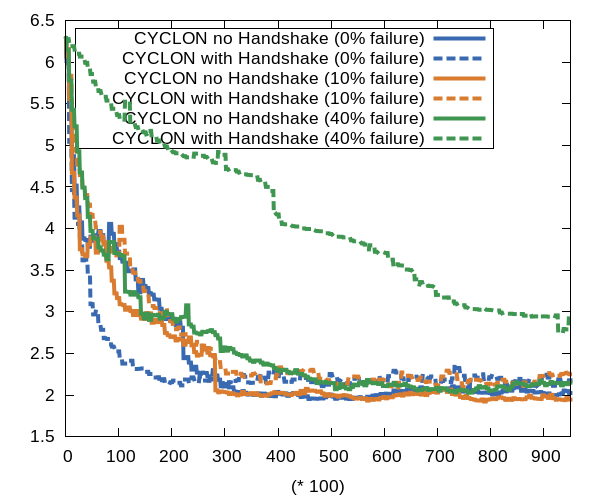
\includegraphics[width=9cm]{Images/statistics/cyclon_1000_c20/avgpath/all}
    \caption{average path length of the CYCLON protocol. }
    \label{fig:path_cyclon}
\end{figure}

Similar to the clustering coefficient, the average path length diverges slower when handshaking is involved.
When the network error rate increases, the handshaking version becomes significantly wider than the non-handshaking one.

Figure \ref{fig:f_scamp1} shows the average path length with SCAMP, run over $100000$ cycles.
Similar to the average cluster coefficient the handshake version degrades quickly when network failures are introduced.

\begin{figure}[H]
    \centering
    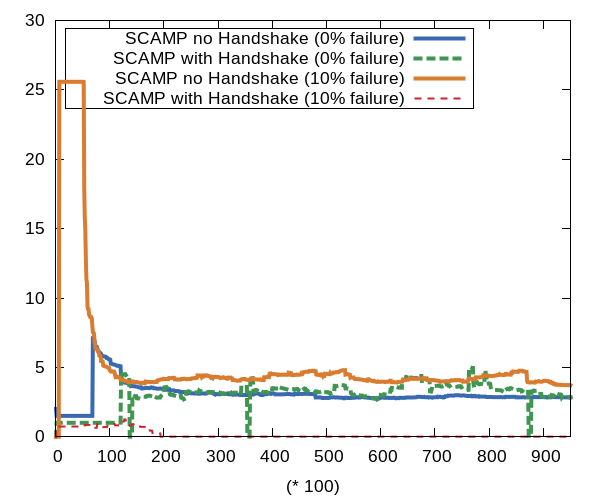
\includegraphics[width=9cm]{Images/statistics/scamp_1000_c2/avgpath/all}
    \caption{average path length of the SCAMP protocol. The y-axis denotes the path length in nodes and the x-axis denotes the number of cycles multiplied by 100.}
    \label{fig:f_scamp1}
\end{figure}

The non-handshaking version handles increasing error rates stabilizing at similar values.
Without network failure, Handshaking SCAMP stabilizes at a similar length as the non-handshaking version - a notable difference are little gaps that sometimes occur that are not present in the non-handshaking variant.


Figure \ref{fig:f_scamp3} shows the connectivity of the SCAMP protocol.
The y-axis denotes the connectivity (ranging from 0 to 1) while the x-axis denotes the number of cycles multiplied by $100$.
SCAMP without handshaking almost always has a high connectivity level - it sometimes drops for a while but recovers shortly after.
When errors are introduced the path length quickly degrades to $0$ suggesting a disconnected graph.

\begin{figure}[H]
    \centering
    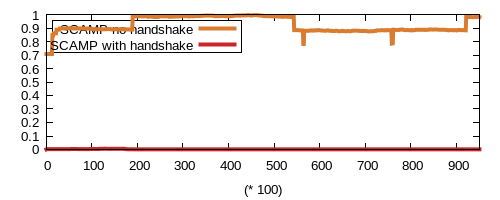
\includegraphics[width=9cm]{Images/statistics/scamp_1000_c2/avgpath/con_10}
    \caption{average connectivity of the SCAMP protocol (10\% failure). The x-axis denotes the number of cycles multiplied by 100 while the y-axis denotes the reaching quota of the network.}
    \label{fig:f_scamp3}
\end{figure}

% REASON

The results mirror those from the \emph{average clustering coefficient}: CYCLON seems to perform very similar with or without handshaking.
Only a significant error rate degrades the handshaking version clearly.
SCAMP on the other hand quickly degrades: the reasons for this stays the same: as the lease and rejoin need to to perform many hops, this also represents many potential sources of error.
Furthermore, as messages travel along the hops they get delayed, thus making nodes waiting for messages to arrive longer than in the non-handshaking version - as we are only evaluating 10 random nodes\footnote{due to performance reasons} out of the network to calculate the average path length this explains the gaps in Figure \ref{fig:f_scamp1}.

\section{SCAMPLON}

SCAMPLON, being a cyclic peer sampling service, naturally shares more similarities and properties with CYCLON than with SCAMP.
Because of that we compare those two protocols. 
The configuration value for SCAMPLON is $c$, which has the same purpose as the $c$ in SCAMP. In this simulation, $c = 3$.
Handshaking will not be used.
As previous experiments have shown, it only adds constant complexity to CYCLON, and, as SCAMPLON shares the same philosophy, this can be transfered to it as well.

\subsection{Average Cluster Coefficient}

Figure \ref{fig:n1} compares the average clustering coefficient from SCAMPLON and CYCLON over the run of $400$ cycles.
We can observer that SCAMPLON delivers a significantly better clustering coefficient than CYCLON when the failure rate is low but when the failure rate exceeds a certain turning point\footnote{In our experiments this was around $23\%$ failure rate} CYCLON starts to yield better results.
The reason for this is that SCAMPLON`s partial view has an almost ideal size of $\log{n}$ while CYCLON`s partial view with a value of $c=20$ exceed this optimum by far thus resulting in a higher interconnection which in turn results in a higher clustering degree.
However, when the failure rate increases, CYCLON outperforms SCAMPLON as it has more links that it can use as backup when others fail.


\begin{figure}[H]
    \centering
    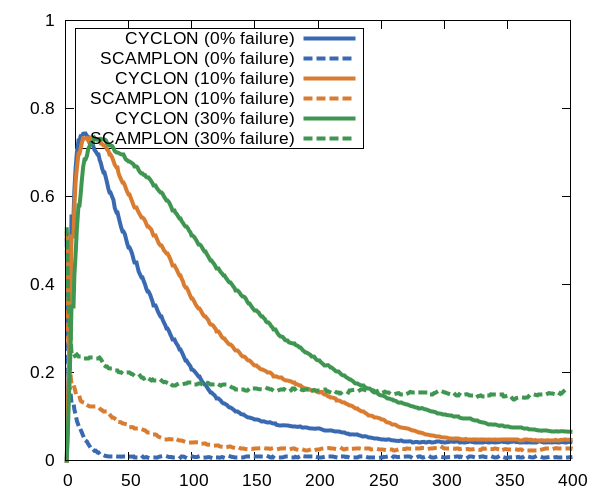
\includegraphics[width=9cm]{Images/statistics/scamplon_1000_c3/cluster/all}
    \caption{average cluster coefficient of the SCAMPLON and the CYCLON protocol. The y-axis denotes the clustering coefficient while the x-axis denotes the number of cycles.}
    \label{fig:n1}
\end{figure}

Another positive property of SCAMPLON is the fast convergence rate\footnote{here after around 25 cycles} which is magnitudes lower than at CYCLON`s.
This can be explained by two properties: first:  smaller partial views saturate faster, and second: SCAMP`s subscription protocol is used for SCAMPLON which results in a better initial distribution of the network thus giving it a head start for the convergence rate.
Figure \ref{fig:n1} underpins this theory as SCAMPLON has a very low maximum value when compared to CYCLON.

\subsection{Average Path Length}

Figure \ref{fig:np} compares the average path length between SCAMPLON and CYCLON.
As we observed previously SCAMPLON converges faster than CYCLON due to the smaller partial views and the better initial distribution thanks to SCAMP`s initialization.

\begin{figure}[H]
    \centering
    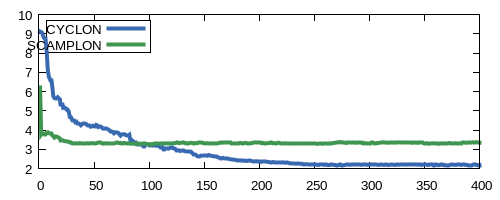
\includegraphics[width=9.3cm]{Images/statistics/scamplon_1000_c3/path_len/p}
    \caption{average path length of the SCAMPLON and the CYCLON protocol. The y-axis denotes the number of hops while the the x-axis denotes the number of cycles.}
    \label{fig:np}
\end{figure}

However, in the long run CYCLON delivers a better average path length.
The reason for this is that CYCLON maintains numerous links more than SCAMPLON and thus is better interconnected with other nodes which in turn results in a lower diameter of the graph.

\subsection{Number of Arcs}

Figure \ref{fig:narc} compares the number of arcs between SCAMPLON and CYCLON.
The y-axis denotes the number of total edges in the graph while the x-axis denotes the time in cycles. 
The result yields no surprise as CYCLON has a bigger partial view and thus is interconnected better and thus has a higher count of arcs.
CYCLON`s arc count converges to $|E_{CYCLON}|\approx c_{CYCLON} * n$.
SCAMPLON on the other hand has a constant number of arcs that are established to $|E_{SCAMPLON}|\approx (c_{SCAMPLON}+1)n\log{n}$ by the initial SCAMP-protocol.
The shuffle function cannot and must not change this value.
A smaller number of arcs has the advantage of reducing the numbers of redundant messages sent in the network thus improving the used bandwidth.
On the other hand, a high count of arcs can result in shorter paths and thus in faster message delivery.
It also improves the resilience against failures.

\begin{figure}[H]
    \centering
    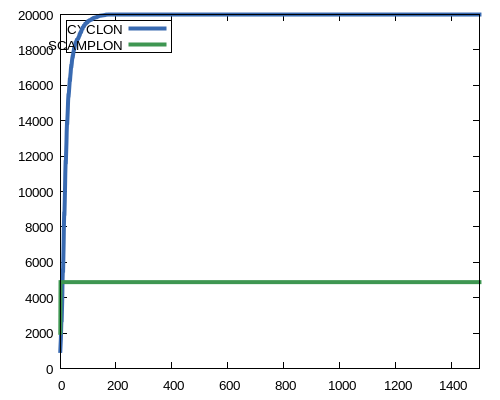
\includegraphics[width=9.3cm]{Images/statistics/scamplon_1000_c3/arc_count/p}
    \caption{Number of arcs in SCAMPLON and CYCLON. The x-axis denotes the time passed in cycles while the y-axis denotes the arc count.}
    \label{fig:narc}
\end{figure}

\section{Conclusion}

We see that our proposed algorithm delivers desirable results which often even exceeds the qualities of CYCLON when the failure rate is low.
Beyond that, SCAMPLON`s adaptive nature gives him additional advantages when compared to traditional cyclic protocols with fixed partial view sizes.
The adaptiveness helps the protocol to be able to virtually always reach the whole network but also to keep the traffic and redundancy low - features that traditional cyclic protocols lack.

However, further research must be conducted to evaluate SCAMPLON`s behavior under churn\footnote{Nodes dynamically leaving and joining the network} to observe the interplay of SCAMP`s subscription protocol with SCAMPLON`s cyclic algorithm.
Additionally, a handshake version must be investigated to validate that the non-handshaking properties can be transfered as it was assumed in this report.
Last, the protocol should be implemented in WebRTC to evaluate it under real network conditions.
The code for the experiments can be found on github\footnote{https://github.com/justayak/peersim-1.0.5}.

%--------------------------------------------------------------------------------

\chapter{Conclusion}

The experiments with SCAMPLON provide good result showing that it is a potential candidate for our WebRTC peer sampling service.
Another good candidate is CYCLON as it can easily be adapted for handshaking with which it performs reliable and robust even with network failures.

\section{Summary}

Our study can be divided in three parts:
First, we wanted to find an efficient and scalable peer sampling service for WebRTC.
As we want to avoid the use of central services as much as possible and instead use local knowledge whenever possible we had to enable the distributed network to fulfill tasks usually handled by a central server.
This task is the handshaking that is mandatory to connect two WebRTC clients with each other.
We implemented handshaking in WebRTC\footnote{https://github.com/justayak/handshake} and concluded that this task can successfully be handled in a distributed manner.

Secondly, we compared two well known peer sampling services, SCAMP and CYCLON, regarding their properties when adapted to handshaking mechanics.
We concluded that CYCLON can handle handshaking fairly well even when in erroneous networks.
SCAMP on the other hand quickly degenerates and thus is not a good choice when handshaking should be executed by the protocol.
However, we found SCAMP`s adaptive view size very desirable as it significantly reduces the messaging overhead when used for information dissemination.

This led to the third step: the creating of SCAMPLON, a cyclic peer sampling service that tries to combine the good properties of SCAMP`s adaptive partial view size, CYCLON`s robustness regarding handshaking and CYCLON`s fast convergence rate.
Our experiments show that SCAMPLON satisfies the desired properties.

\section{Outcomes}

The outcome of our research is the new cyclic peer sampling algorithm SCAMPLON.
It combines the two protocols SCAMP and CYCLON, is simple and, most of the time, it makes use of peers with close proximity making it a good candidate for a handshaking WebRTC environment.

\section{Research directions}

Further research must be devoted to SCAMPLON`s behavior under churn.
Additionally, we must evaluate how the failure of full nodes affect the network as there is no lease mechanism to repair the overall structure.
So far, the unsubscription was not tested which is an important part of the protocol.
And, least, the protocol must be implemented in WebRTC to see how it behaves under network conditions.

%--------------------------------------------------------------------------------

\nocite{*} % to be removed, actual citations in the report must be necessary and sufficient (this is just to create a fake bibliography in the model)

\bibliography{rapport}

\listoffigures{}

\listoftables{}

\listofalgorithms{}

\appendix

\chapter{Annotated References}
\label{app:FichesLecture}

\paragraph{\emph{CYCLON: Inexpensive Membership Management for Unstructured P2P Overlays}.}

Describe rapidly what problem is attacked in the paper (add the reference, e.g. \cite{Voulgaris05cyclon:inexpensive}).

\subparagraph{Summary.}

The summary presents the main idea of the paper and the work conducted \emph{by the authors} up to their conclusions.

\subparagraph{Analysis.}

It is only during a second phase that you can analyse the contents of the paper, i.e., verify it (errors are always possible in the scientific literature!), express your opinion about the advances claimed by the paper, and establish a connection with your own work.

\paragraph{\emph{Title of a paper}.}

Etc.

\chapter{Schedule}

This appendix is \emph{mandatory}.

Figure~\ref{fig:Drafting} shows the draft schedule establish \emph{a priori}\ldots

\begin{figure*}
% - Use the starred version in order to put floats on two columns
% - Possibly, use the "\ifscreen ... \else ... \fi"" alternative to orientate correctly
%   the planning with respect to the orientation of the paper (cf. below for the auto-evaluation)
   \centering
      \emph{<Insert a Gantt's diagram.>}
   \caption{Drafting}
   \label{fig:Drafting}
\end{figure*}

Figure~\ref{fig:Planning} introduce the planning that has been build week after week during the course of the work.

\begin{figure*}
   \centering
      \emph{<Insert a Gantt's diagram.>}
   \caption{Planning}
   \label{fig:Planning}
\end{figure*}

Discuss differences between the drafting and the planning as well as lessons learned on the management of a research project or R\&D project.

\chapter{Weekly Reports}
\label{ann:WeeklyReports}

This appendix is \emph{mandatory}.

\begin{fichesuivi}{September 13, 2010}{September 18, 2010}
   \tempstravailA{2}{30}
   \tempstravailB{3}{45}

   \begin{travaileffectue}
      \begin{itemize}
         \item Task 1:  difficulty, simplicity; achieved, advanced up to $t$\%; etc.;
         \item Task 2:  \ldots;
         \item Etc.
      \end{itemize}
   \end{travaileffectue}

   \begin{travailnoneffectue}
      \begin{itemize}
         \item Task 1:  reasons; postponements, cancellations; etc.;
         \item Task 2:  \ldots;
         \item Etc.
      \end{itemize}
   \end{travailnoneffectue}

   \begin{echange}
      \begin{itemize}
         \item Questions;
         \item Answers;
         \item Clarification, comprehension;
         \item Choices, orientations, reorientations;
         \item Etc.
      \end{itemize}
   \end{echange}

   \begin{planification}
      \begin{itemize}
         \item Researches to be conducted;
         \item Papers to be read, understood, and analysed;
         \item Codes to develop;
         \item Etc.
      \end{itemize}
   \end{planification}
\end{fichesuivi}

\begin{fichesuivi}{September 20, 2010}{September 24, 2010}
   \tempstravailA{7}{50}
   \tempstravailB{5}{45}

   \begin{travaileffectue}
   \end{travaileffectue}

   \begin{travailnoneffectue}
   \end{travailnoneffectue}

   \begin{echange}
   \end{echange}

   \begin{planification}
   \end{planification}
\end{fichesuivi}

\begin{fichesuivi}{September 27, 2010}{October 1st, 2010}
   \tempstravailA{11}{20}
   \tempstravailB{9}{55}

   \begin{travaileffectue}
   \end{travaileffectue}

   \begin{travailnoneffectue}
   \end{travailnoneffectue}

   \begin{echange}
   \end{echange}

   \begin{planification}
   \end{planification}
\end{fichesuivi}

\begin{fichesuivi}{}{}
   \tempstravailA{14}{30}
   \tempstravailB{9}{20}

   \begin{travaileffectue}
   \end{travaileffectue}

   \begin{travailnoneffectue}
   \end{travailnoneffectue}

   \begin{echange}
   \end{echange}

   \begin{planification}
   \end{planification}
\end{fichesuivi}

\begin{fichesuivi}{}{}
   \tempstravailA{12}{30}
   \tempstravailB{3}{40}

   \begin{travaileffectue}
   \end{travaileffectue}

   \begin{travailnoneffectue}
   \end{travailnoneffectue}

   \begin{echange}
   \end{echange}

   \begin{planification}
   \end{planification}
\end{fichesuivi}

\begin{fichesuivi}{}{}
   \tempstravailA{7}{10}
   \tempstravailB{14}{30}

   \begin{travaileffectue}
   \end{travaileffectue}

   \begin{travailnoneffectue}
   \end{travailnoneffectue}

   \begin{echange}
   \end{echange}

   \begin{planification}
   \end{planification}
\end{fichesuivi}

\begin{fichesuivi}{}{}
   \tempstravailA{9}{15}
   \tempstravailB{13}{45}

   \begin{travaileffectue}
   \end{travaileffectue}

   \begin{travailnoneffectue}
   \end{travailnoneffectue}

   \begin{echange}
   \end{echange}

   \begin{planification}
   \end{planification}
\end{fichesuivi}

\begin{fichesuivi}{}{}
   \tempstravailA{18}{40}
   \tempstravailB{1}{25}

   \begin{travaileffectue}
   \end{travaileffectue}

   \begin{travailnoneffectue}
   \end{travailnoneffectue}

   \begin{echange}
   \end{echange}

   \begin{planification}
   \end{planification}
\end{fichesuivi}

\begin{fichesuivi}{}{}
   \tempstravailA{21}{40}
   \tempstravailB{17}{10}

   \begin{travaileffectue}
   \end{travaileffectue}

   \begin{travailnoneffectue}
   \end{travailnoneffectue}

   \begin{echange}
   \end{echange}

   \begin{planification}
   \end{planification}
\end{fichesuivi}

\begin{fichesuivi}{}{}
   \tempstravailA{4}{30}
   \tempstravailB{8}{15}

   \begin{travaileffectue}
   \end{travaileffectue}

   \begin{travailnoneffectue}
   \end{travailnoneffectue}

   \begin{echange}
   \end{echange}

   \begin{planification}
   \end{planification}
\end{fichesuivi}

\begin{fichesuivi}{}{}
   \tempstravailA{10}{10}
   \tempstravailB{11}{00}

   \begin{travaileffectue}
   \end{travaileffectue}

   \begin{travailnoneffectue}
   \end{travailnoneffectue}

   \begin{echange}
   \end{echange}

   \begin{planification}
   \end{planification}
\end{fichesuivi}

\begin{fichesuivi}{}{}
   \tempstravailA{3}{30}
   \tempstravailB{2}{10}

   \begin{travaileffectue}
   \end{travaileffectue}

   \begin{travailnoneffectue}
   \end{travailnoneffectue}

   \begin{echange}
   \end{echange}

   \begin{planification}
   \end{planification}
\end{fichesuivi}

\begin{fichesuivi}{}{}
   \tempstravailA{10}{00}
   \tempstravailB{10}{00}

   \begin{travaileffectue}
   \end{travaileffectue}

   \begin{travailnoneffectue}
   \end{travailnoneffectue}

   \begin{echange}
   \end{echange}

   \begin{planification}
   \end{planification}
\end{fichesuivi}

\begin{fichesuivi}{}{}
   \tempstravailA{3}{45}
   \tempstravailB{10}{20}

   \begin{travaileffectue}
   \end{travaileffectue}

   \begin{travailnoneffectue}
   \end{travailnoneffectue}

   \begin{echange}
   \end{echange}

   \begin{planification}
   \end{planification}
\end{fichesuivi}

\begin{fichesuivi}{}{}
   \tempstravailA{16}{30}
   \tempstravailB{18}{15}

   \begin{travaileffectue}
   \end{travaileffectue}

   \begin{travailnoneffectue}
   \end{travailnoneffectue}

   \begin{echange}
   \end{echange}

   \begin{planification}
   \end{planification}
\end{fichesuivi}

\begin{fichesuivi}{}{}
   \tempstravailA{14}{30}
   \tempstravailB{22}{30}

   \begin{travaileffectue}
   \end{travaileffectue}

   \begin{travailnoneffectue}
   \end{travailnoneffectue}

   \begin{echange}
   \end{echange}

   \begin{planification}
   \end{planification}
\end{fichesuivi}

\begin{fichesuivi}{}{}
   \tempstravailA{17}{45}
   \tempstravailB{12}{50}

   \begin{travaileffectue}
   \end{travaileffectue}

   \begin{travailnoneffectue}
   \end{travailnoneffectue}

   \begin{echange}
   \end{echange}

   \begin{planification}
   \end{planification}
\end{fichesuivi}

\begin{fichesuivi}{}{}
   \tempstravailA{13}{10}
   \tempstravailB{9}{30}

   \begin{travaileffectue}
   \end{travaileffectue}

   \begin{travailnoneffectue}
   \end{travailnoneffectue}

   \begin{echange}
   \end{echange}

   \begin{planification}
   \end{planification}
\end{fichesuivi}

The summary table of work dedicated to the project is \emph{mandatory}.
If you do not use the provided weekly report sheets, you must establish the summary by yourself.
Otherwise, the simple command that follows in the source code (\verb+\printweeksummary+) does all the job of generating the table along with all the hyperlinks to the weekly reports.

\printweeksummary

\chapter{Self-assessment}

This appendix is \emph{mandatory}.

Figure~\ref{fig:IntermediateAutoEvaluation} enumerates a number of important points related to the three aspects of the work:
\begin{enumerate}
   \item report;
   \item oral presentation;
   \item results.
\end{enumerate}
This allows to evaluation your own level of satisfcation at the end of the first part of the project, consisting of:
\begin{enumerate}
   \item preliminary study;
   \item bibliographic study;
   \item general design of a solution.
\end{enumerate}

You can discuss in some details these various points.

\begin{figure*}
   \centering
      \ifscreen % macro TeX (issue de la classe report-rd-info.cls) permettant d'ajuster le contenu en fonction du l'orientation du document (<< screen >> ou pas)
         \rotatebox{90}{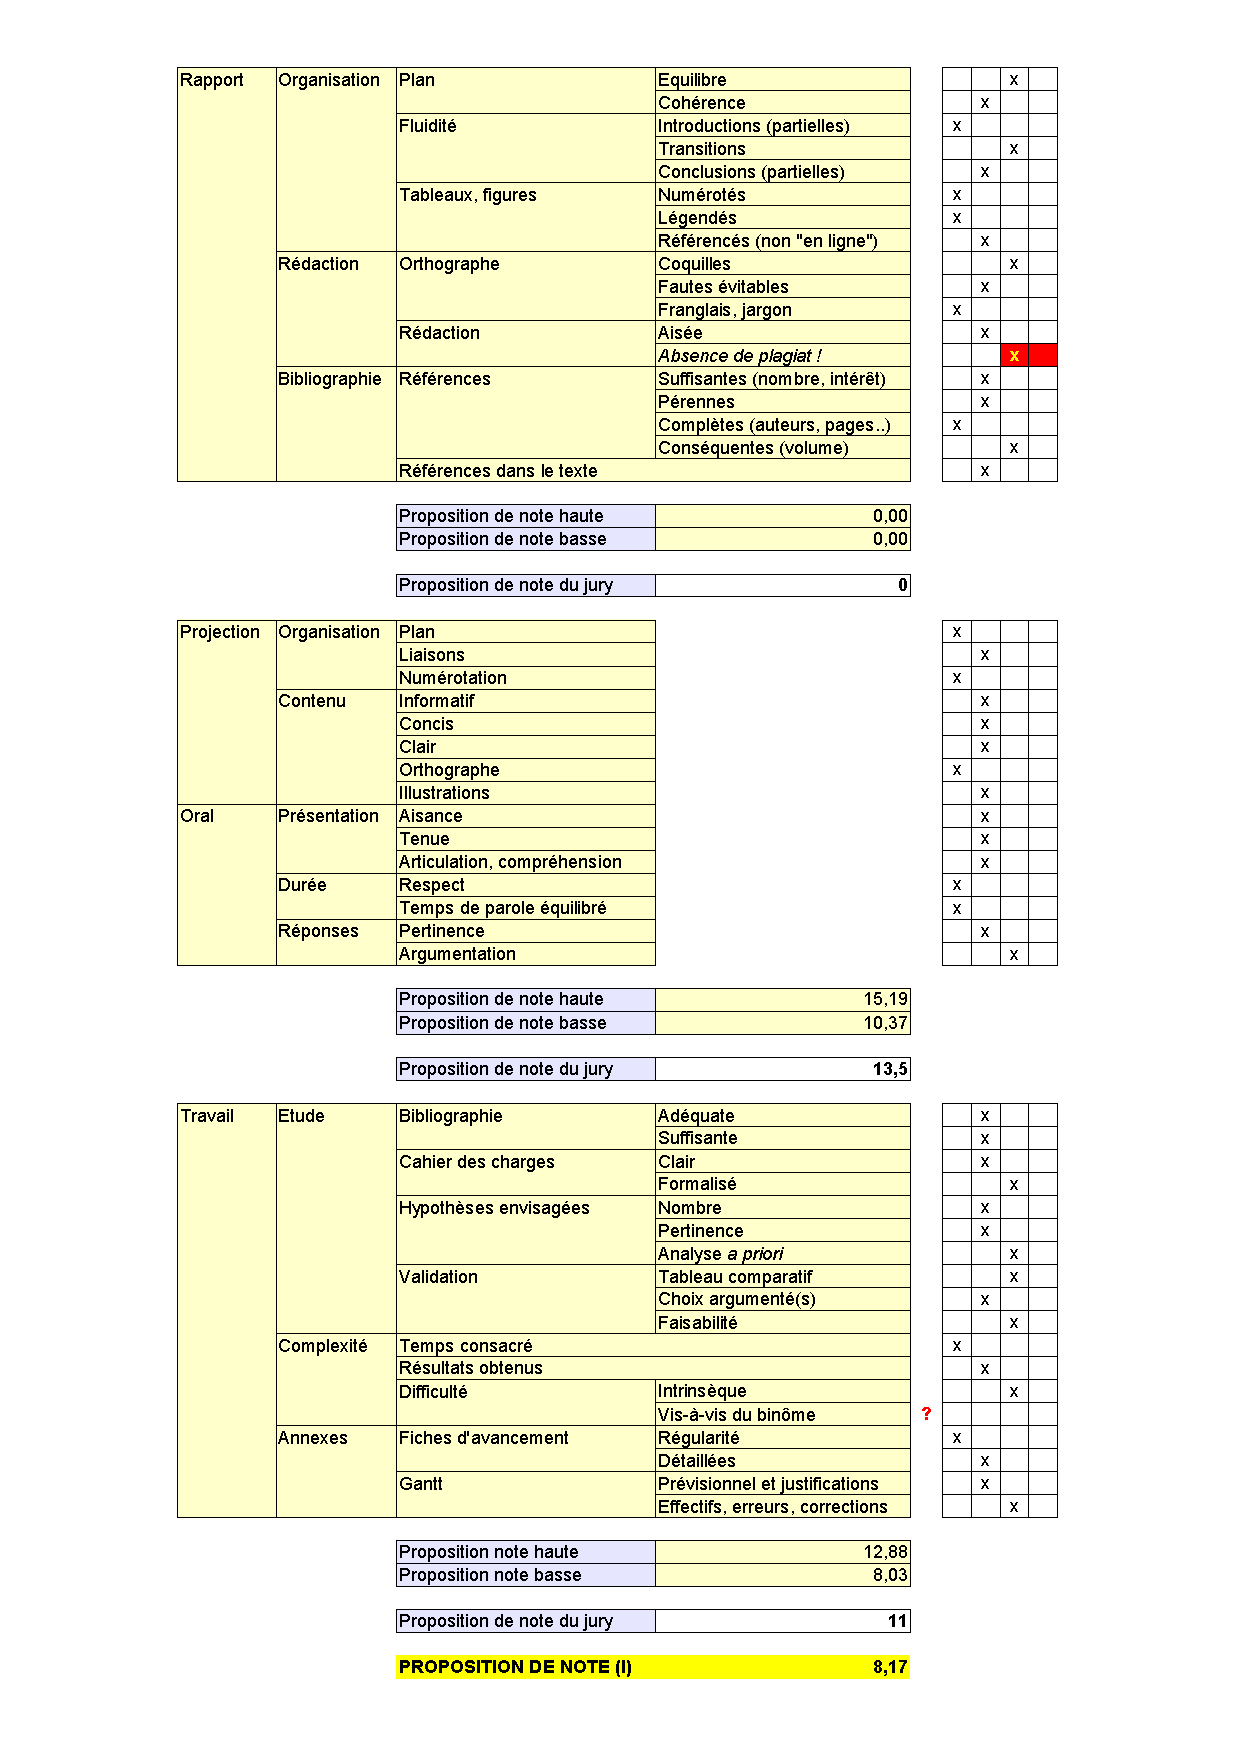
\includegraphics[width=0.9\textheight]{Images/Grille-Evaluation-PRD1}}
      \else
         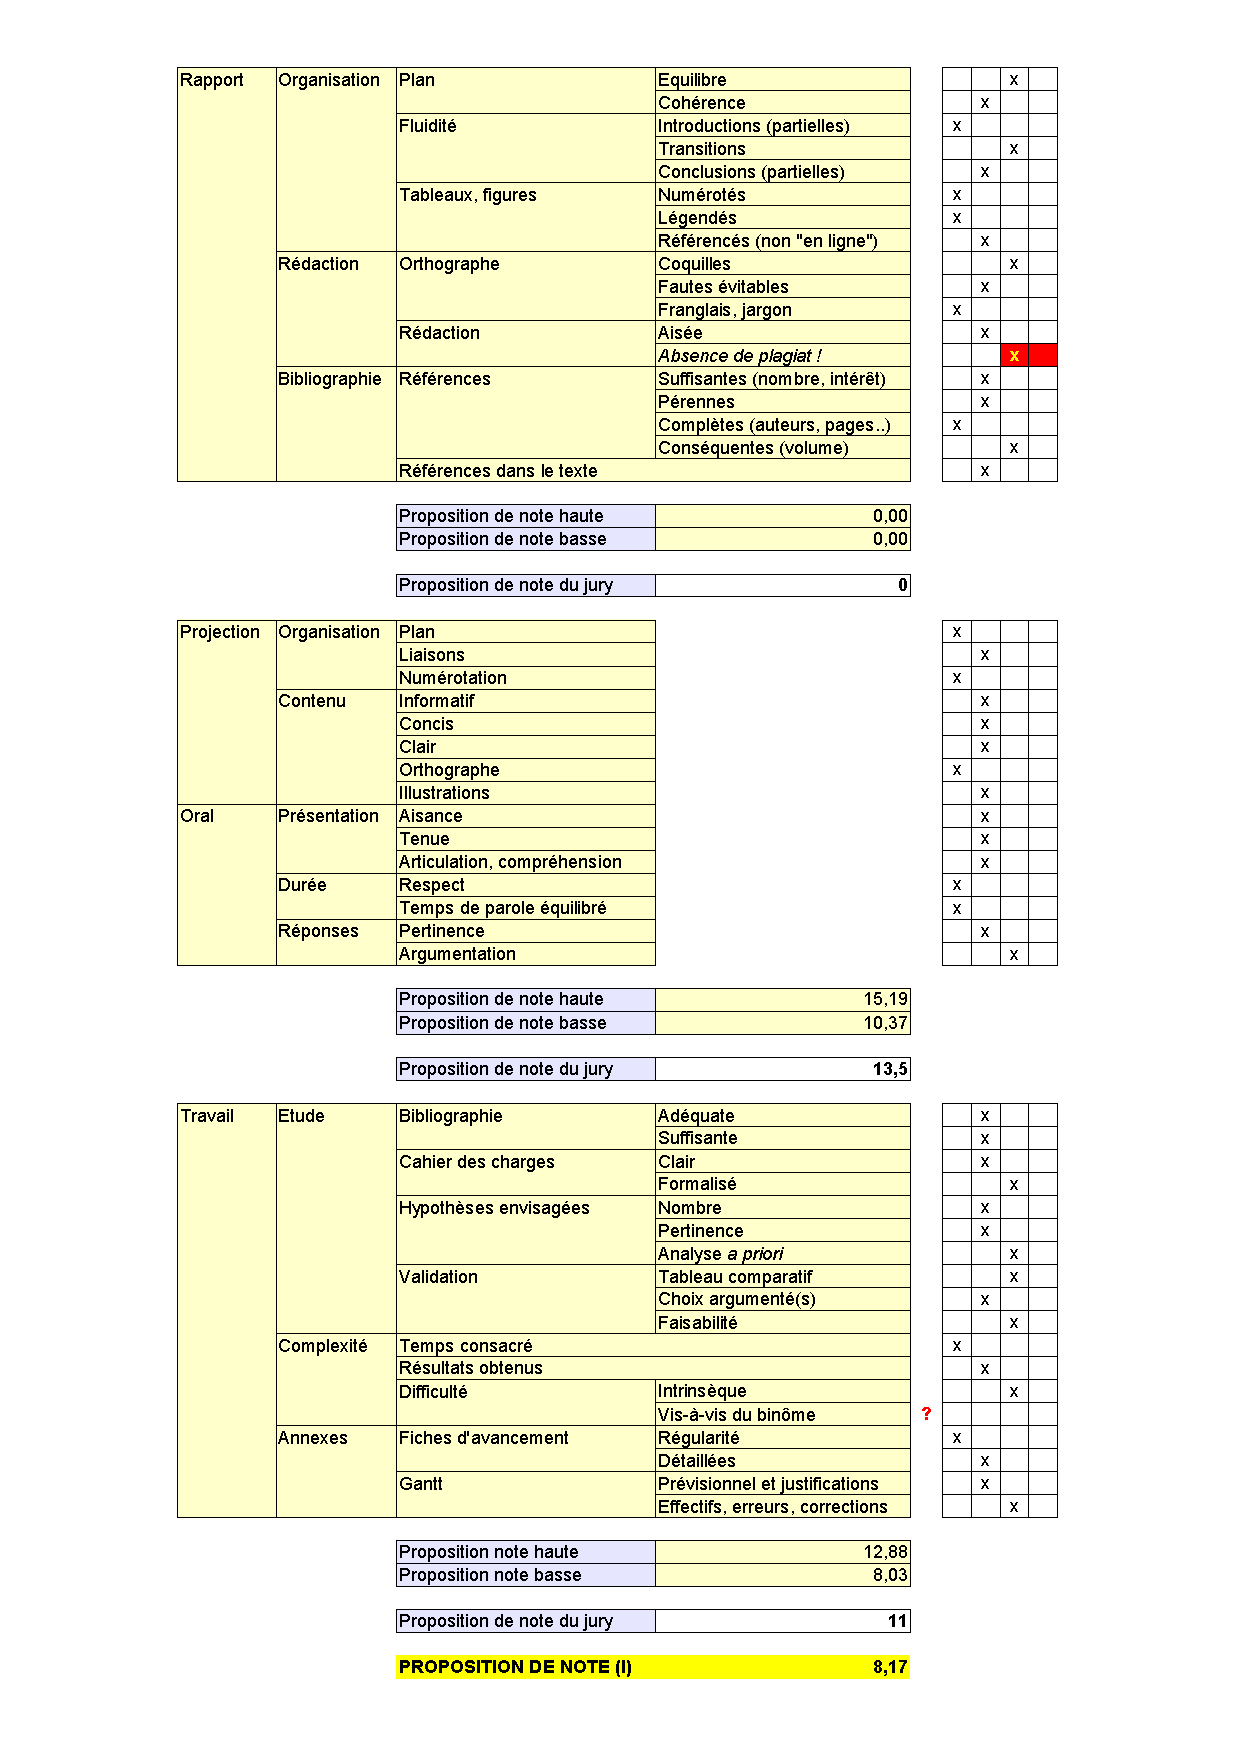
\includegraphics[width=0.9\textwidth]{Images/Grille-Evaluation-PRD1}
      \fi
   \caption{Points � contr�ler � l'issue de la phase I}
   \label{fig:IntermediateAutoEvaluation}
\end{figure*}

Figure~\ref{fig:FinalAutoEvaluation} provides the same kind of evaluation for the second part of the project, i.e.:
\begin{enumerate}
   \item detailed design;
   \item development;
   \item receipt.
\end{enumerate}

\begin{figure*}
   \centering
      \ifscreen
         \rotatebox{90}{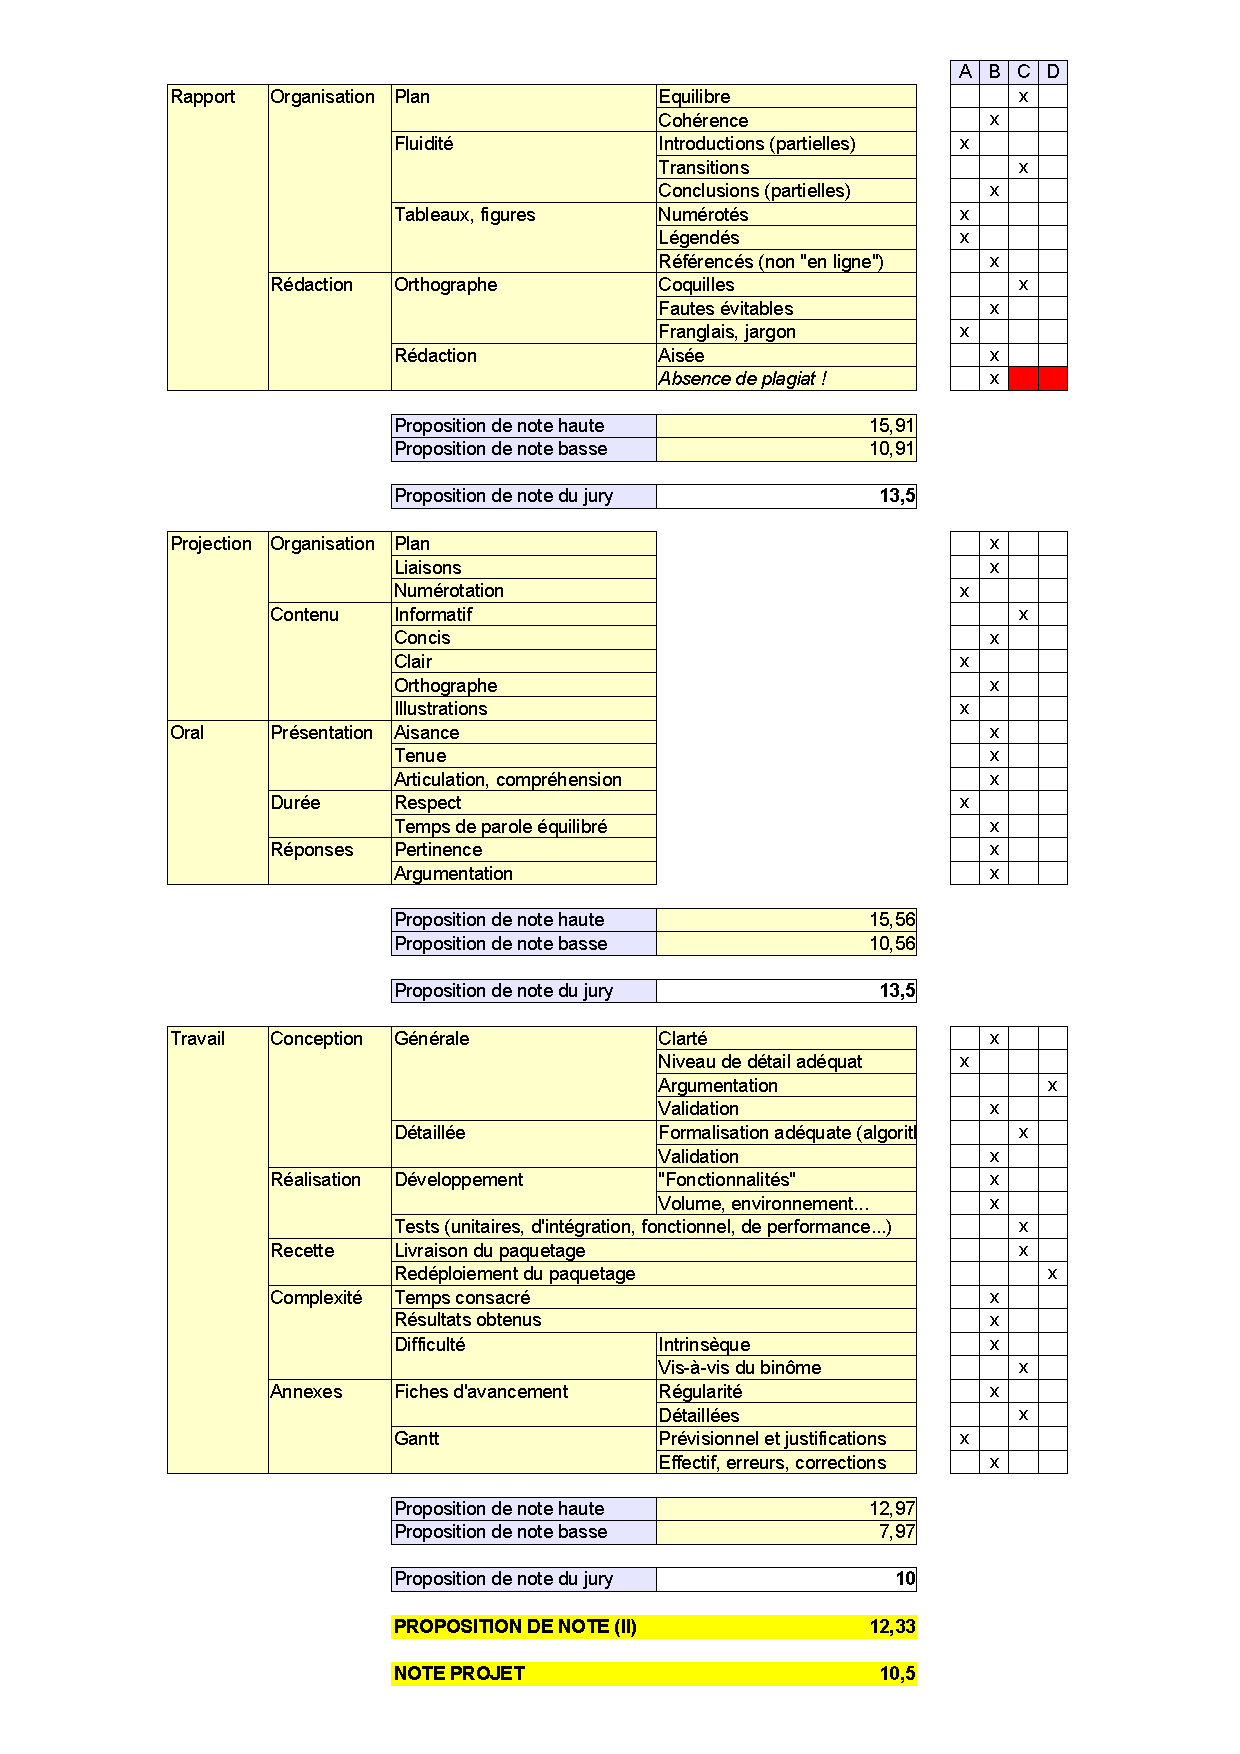
\includegraphics[width=0.9\textheight]{Images/Grille-Evaluation-PRD2}}
      \else
         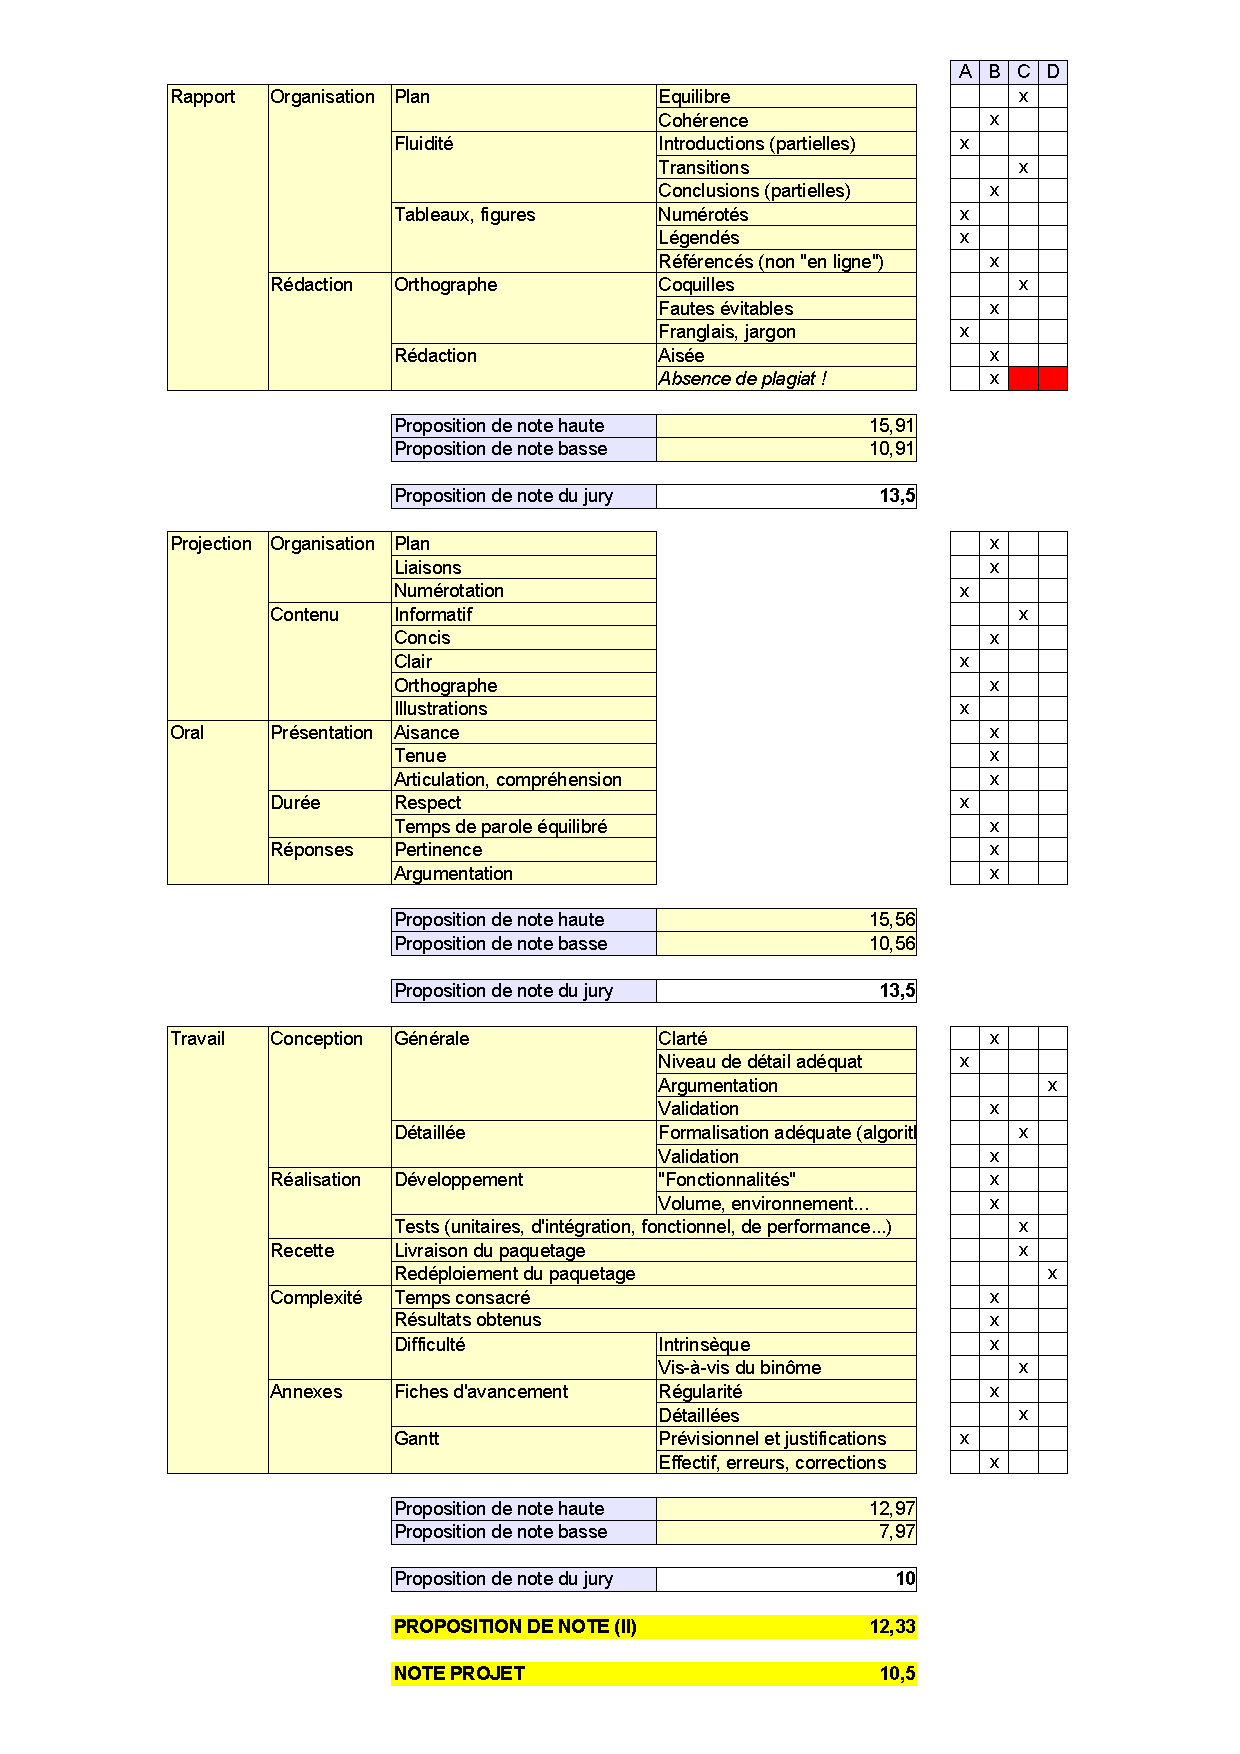
\includegraphics[width=0.9\textwidth]{Images/Grille-Evaluation-PRD2}
      \fi
   \caption{Points � contr�ler � l'issue de la phase II}
   \label{fig:FinalAutoEvaluation}
\end{figure*}

\end{document}
